\documentclass [12pt]{article}
\usepackage{fancyhdr}
\usepackage[utf8]{inputenc}
\usepackage[english]{babel}
\usepackage{gensymb}
\usepackage{amsmath,amssymb,amsfonts}
\usepackage{algorithmic}
\usepackage{graphicx}
\usepackage{textcomp}
\usepackage[table]{xcolor}
\usepackage{siunitx}
\usepackage{indentfirst}
\usepackage[margin=2.5cm]{geometry}
\usepackage{float}
\usepackage{hyperref}
\usepackage[UKenglish]{datetime}
\usepackage{setspace}
\usepackage{hhline}
\usepackage{lastpage}
\usepackage[numbers]{natbib}
\usepackage[acronym]{glossaries}
\usepackage{listings}
\usepackage{color}
\usepackage{booktabs}% http://ctan.org/pkg/booktabs
\newcommand{\tabitem}{~~\llap{\textbullet}~~}
\usepackage{subfigure}

\usepackage{helvet}
\renewcommand{\familydefault}{\sfdefault}

\definecolor{customgreen}{rgb}{0,0.6,0}
\definecolor{customgray}{rgb}{0.5,0.5,0.5}
\definecolor{custommauve}{rgb}{0.6,0,0.8}

\graphicspath{{images/}}

\hypersetup
{
    colorlinks=true,
    linkcolor=black,
    urlcolor=blue,
}

\doublespacing

\begin{document}

\title{\bf Report Title}
\author{Daniel Cole, Jack Pendlebury, Noah Harvey, Luke Waller}
\date{\today}
\maketitle
\thispagestyle{empty}

\newpage
\fancyfoot[R]{Page \thepage \hspace{1pt} of \pageref{LastPage}}
\setcounter{page}{1}
\pagenumbering{arabic}
\tableofcontents
\newpage

\listoffigures
\listoftables

\newpage
\section{Team Organisation}\label{sec:Team_Organisation}

\subsection{Tasking}\label{sec:Tasking}

The tasking is delegated on a Kanban board, with a description of the planned action items and a completion deadline. As the project had an industrial sponsor, this task log was used to implement additional requirements. These focused more on the who, what, and why questions that arose from collaborating directly with a customer. The incorporation of the Kanban board into the Microsoft Teams enabled notifications and reminders for task deadlines and increased the efficiency due to being inside of the Teams channel. 

\subsection{Leadership and Team Organisation}\label{sec:Leadership_and_Team_Organisation}

The leadership approach used in this project is democratic, drawing upon individual’s knowledge and skills in relation to decisions. Democracy ensures that all four members are heard as equals, with the role of the leader within the group alternating when meetings are held. This method has benefited the project by allowing each member to influence the operational style of meetings, providing an opportunity to explore alternative methods of delivery. Elements of affiliative leadership have been utilised to focus on building relationships and facilitating communication. An example if this refers to a situation where illness affected the performance of a member, and upon returning to work they required an additional meeting to reintroduce themselves back into their role. The purpose of this meeting was to discuss the week’s progress, understand the decisions that had been made during the absence and facilitate their incorporation back into the team’s changed environment. 

\subsection{Team Member Roles and Responsibilities}\label{sec:Team_Member_Roles_and_Responsibilities}

\begin{figure}[H]
\centerline{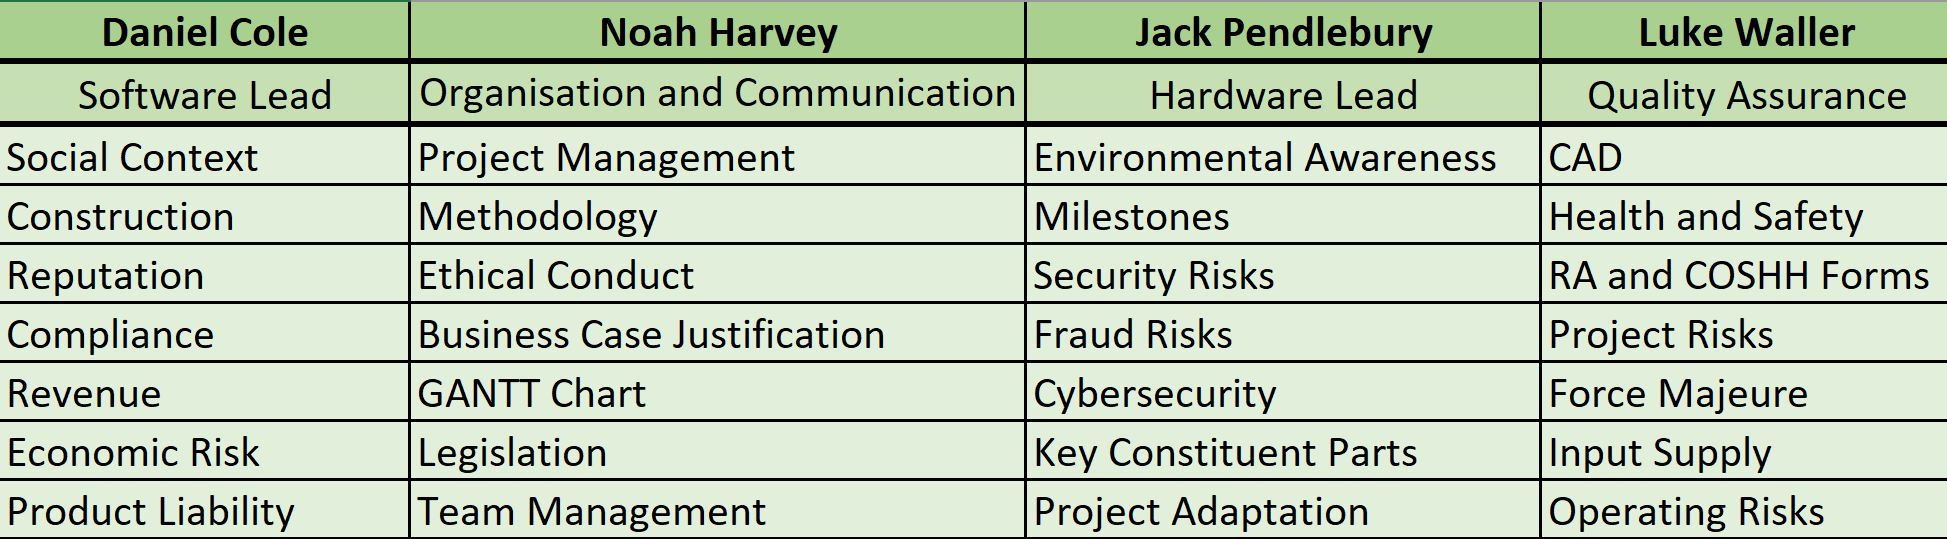
\includegraphics[width=1\textwidth]{TeamRoles.png}}
\caption{Team member roles and responsibilities}
\label{fig:figure_1}
\end{figure}

\textbf{Jo Byrne} is the employer engagement supervisor and the manager for the ESF Smart Specialisation project. Her role within this project is to facilitate liaison between Sirmon and the sponsorship scheme to ensure that, as a customer, Sirmon are satisfied with the performance of HEVCS. Jo attends and schedules regular meetings with the team and Sirmon both together and individually. 
\\
\textbf{Jake Gibson Shaw-Sutton} is the project supervisor who attends meetings with the immediate project team and with Sirmon Industries. 
\\
\textbf{Paul Davey} is the module lead, requiring project overview meetings monthly. He holds the authority to approve health and safety risk assessments, COSHH forms and access to the project budget. 
\\
\textbf{Sirmon Industries}, consisting of Heather and James Sirmon, are the sponsors of the HEVCS project. The specification was written with their requirements for the product, and so they have a higher level of influence in the project and the tasking. The development cycles, stage boundaries and milestones were written in accordance with the scope the team defined during meetings with Jake and Jo.

\subsection{Meeting Structure}\label{sec:Meeting_Structure}

Another main principle of the agile methodology used is that the customer and developers work together daily throughout the project. The team will meet every Tuesday and Friday to discuss the tasking and research development for individual members. Involvement from the customer is paramount, with all advances within the project's operations reported and made accessible on the team's channel. Advantages of regular contact include the minimisation of confusion, specifications, and the incorporation of everybody's goals. 
\\
With face-to-face conversation being the most efficient way of discussing the project, the team meet weekly with the customer on Zoom or in person. Conversing in this manner benefits the customer as they can bear witness to the achievements and provide feedback instantly. Additionally, emails are used to transfer documents for review and discussion, and group chats enable instant messages to be received. For this project, the group chat has been vital for planning, acknowledgement of receipt of documents and daily updates. The digital record of communication also provides accountability for both parties, in the event of a dispute. 
\\
Project related research will be carried out throughout the week, with write ups and findings being reported to the entire team every Monday morning. This way, any problems, such as incomplete tasks or actions from previous meetings, have been highlighted and discussed at the start of the working week. Tuesday afternoons will be used to facilitate group efforts to overcome problems and employ the tools and methods necessary.
\\ 
Bi-weekly meetings will be held with Sirmon Industries, our supervisor (Jake) and the employment engagement officer (Jo). These meetings are used to discuss project progress in detail to facilitate accomplishing both academic and industry criteria. In semester 2, these meetings with Sirmon will run every week.
\\
Fridays will allow the team to come together and reflect upon the week. All team members will provide an overview of their week, how they felt about the tasks they completed and how the team’s approach could be altered for the following week. This will involve confirming availability, especially as other aspects of the module begin to take precedence of the Tuesday afternoon timetabled sessions.



\section{Comercial Risk Evaluation}\label{sec:Commercial_Risk}

\subsection{Security and Fraud}\label{sec:Security_and_Fraud}

Commercial Fraud is not a crime within itself in the eyes of English law, however there are numerous actions that can constitute fraud. These include but are not limited to fraudulent misrepresentation or deceit; conspiracy; inducing a breach of contract; bribery; certain breaches of fiduciary duty; breach of trust, for example dishonest assistance; and claims for wrongful or fraudulent trading under the Insolvency Act 1986.
\\
Some examples of these actions are things such as the misappropriation of assets and funds and overstating expense and budgetary claims. These risk factors can be mitigated through thorough bookkeeping and holding team members accountable for purchases using the budget. Every purchase using the budget should be agreed upon unanimously before having the purchase order sent off for consideration. Each purchase order will additionally be verified at the other end, whether by the university stores or the company sponsor. This two-layer verification will stop any fraudulent behaviour – intentional or otherwise.
\\
Other types of fraud listed above are less applicable to the sponsor-student relationship that this project revolves around, and furthermore are covered within the University’s Student Charter. Breaches of this hold severe academic consequences, and the team members will be encouraged to report any potential breaches to the relevant parties, such as the project supervisors, module leaders, and faculty staff.
\\
Cybersecurity attacks continue to increase year-on-year, despite a growing reliance on technology and cloud-based solutions for common services. 2022 saw a particularly large vulnerability exploited in the Apache web server software, as well as a significant increase in cyber-warfare attacks directed from within the Russo-Ukrainian conflict. This has only added to the increase in the number of attacks, and corporate entities everywhere are being encouraged to take further measures to secure their assets.
\\
By far the most common attack vector is through compromised account credentials. The project’s sensitive code will be stored in a private Git repository, and team members will be encouraged to take action to secure their own accounts with unique passwords and two-factor authentication. GitHub is considered secure, the largest breaches being due to authorisation tokens stolen at the company level, as opposed to server-side breaches. 
\\
Similar precautions will be taken for OneDrive. OneDrive will function as a secure cloud storage location for project materials, such as risk assessments, execution plans, methodology reports, and other such materials. OneDrive shares the same vulnerabilities that GitHub does regarding the weakest link being the human layer. As previously stated, team members will be encouraged to use unique passwords, and access will only be given to team members and university staff on a need-to-know basis.
Materials graded confidential will never be shared beyond the team and relevant staff, and any public release of confidentially graded material must be authorised by the sponsor first. This release will be kept to the bare minimum, and any information within a document to be released that is not authorised will be redacted.

\subsection{Construction}\label{sec:Construction_Risk}

Construction risks are the risks to the construction phase of the project. These risks can range in type, from materials not arriving on time to components being damaged on arrived (DOA). These risks are easy to mitigate against using various methods. It is import for a project with such tight time resections that the components are not ordered using a just in time (JIT - https://www.planview.com/resources/guide/what-is-lean-manufacturing/just-in-time-manufacturing/) manner. For a project of this nature, it is important that the materials are obtained well in advance of needing them just in case there are only issues that could cause a significant delay. This also ensures any issues with the components can be sorted well within the margins of safety of construction time for the project.
\\ 
Drying/Curing/Hardening times are also important to consider when evaluating the construction timeline for the project. It is important to evaluate this to make sure that time is not being spent waiting for assemblies to dry.
\\
Some instances of construction risks are outlined below: 

\begin{itemize}
    \item Materials not arriving on time (being delayed)
    \item Damage to components and parts
    \item Delays in received machined/cut parts delaying construction
    \item Drying/curing/hardening times
\end{itemize}

\subsection{Compliance}\label{sec:Compliance_Risk}

When a company begins a project, they will have to make sure that they are complying with all relevant legislation. If regulations outlined within the legislation are not met, then there could be financial or legal penalties. To make sure that the HEVCS platform can be used on pavements, the team are making sure that it will keep to the legislation pertaining to class 2 mobility scooters. This legislation describes the max weight, dimensions, and the max speed that the platform can be. The team will also make sure that any batteries that they use will comply with the safety standards set in the UK. Legislation will be regularly consulted, and any adjustments made to keep the platform within the requirements. Product safety standards

\subsection{Revenue}\label{sec:Revenue_Risk}

Revenue can be affected by a range of risks, including operational, reputation, economic, competition and force majeure. If precautions haven’t been put into place for these risks, the revenue of the project may be negatively impacted. Each risk has been evaluated and steps to alleviate them have been put into place.
\\
Reputation of the company has the potential of impacting a project financially, either positively or negatively. Damages to reputation can come from actions that can be discourteous or incompetent. The main potential for this project to gain negative publicity will come from either: the team saying or posting something online which paints Sirmon Industries in a negative light, or the final product being built to poor standards. To prevent these issues, the team will be careful with what they post online or what they say to potential customers. making sure that they do not accidently create any adverse view towards Sirmon Industries. To make sure the HEVCS platform is made to the best quality possible, the team will extensively research each possible component and select based on quality and budget of the project.
\\
Competing companies could develop a product that encroaches on the HEVCS platform, decreasing the demand for it and potentially reducing the prospective revenue. Also, companies might already have a product that solves the same problem as the HEVCS platform. To make sure that this does not happen, the team have researched IPs to make sure that the HEVCS platform will not infringe on any other product.
\\
With the fluctuation of the market constantly affecting the economy, a project will be met with some economic risk. Currently, the UK is facing an economic crisis, with inflation being at a 30-year high and the country having entered a recession. To try and mitigate any risk that might arise from these economic changes, the team will keep approximately £500 of the budget in reserve, to absorb any potential cost fluctuations.   
\\
Operating Risks are the risks resulting from ineffective or failed internal processes, systems, people, or external events that may cause disruption to the flow of business operations. These risks can be due to Employee error, criminal activity such as fraud, and even physical events. These can all trigger operational risks. 
\\
Examples of Operating risks are outlined below:

\begin{itemize}
    \item Ineffective Communication between members of the team or between the project team and Sirmon Industries
    \item Not being able to afford the best components causing failures and setbacks within the project
    \item Inflation causing all components to become more expensive to purchase
    \item Scope creep
\end{itemize}

Construction risks are the risks to the construction phase of the project. These risks can range in type, from materials not arriving on time to components being damaged on arrived (DOA). These risks are easy to mitigate against using various methods. It is import for a project with such tight time resections that the components are not ordered using a just in time \cite{Just-In-Time_Manufacturing} manner. For a project of this nature, it is important that the materials are obtained well in advance of needing them just in case there are only issues that could cause a significant delay. This also ensures any issues with the components can be sorted well within the margins of safety of construction time for the project. 
Drying/Curing/Hardening times are also important to consider when evaluating the construction timeline for the project. It is important to evaluate this to make sure that time is not being spent waiting for assemblies to dry.
Some instances of construction risks are outlined below:

\begin{itemize}
    \item Materials not arriving on time (being delayed)
    \item Damage to components and parts
    \item Delays in received machined/cut parts delaying construction
    \item Drying/curing/hardening times
\end{itemize}

\subsection{Project}\label{sec:Projcet_Risk}

Project risks outline any person/interpersonal issues that may arise during the project. These risks are hard to mitigate against and can happen at any point. Because these risks are unavoidable and unplanned, a contingency plan must be always in place just in case any issues may arise. 
\\
Contingency plans include, moving meetings to an online format in case of unavailability of persons to attend meetings in person. Reschedule meetings for when all attendees are available. Understand the workloads of everyone within the team so if a member is unable to continue working for a certain time. This would allow other team members to reassign tasks accordingly.

\begin{itemize}
    \item Someone falls ill/gets covid
    \item Family emergencies
    \item Personal economic disaster (someone can no longer afford to study at university)
\end{itemize}

\subsection{Input Supply}\label{sec:Input_Supply_Risk}

Input Supply risks are risks involving the obtaining of materials and components that are needed for the project. It encapsulates the sourcing and arrival of components and how this may affect the progress made on a project. In the current economic climate supply chains have been drastically affected; they are unable to continue to supply the needed number of components. Due to the high demand and short supply, components are becoming more expensive and more difficult to obtain. The supply shortage has many contributing factors such as, the worldwide silicone shortage, the COVID-19 pandemic, and the on-going war in Ukraine. 
\\
Although parts of supply chains are beginning to see a return towards normality, there are still major disruptions on many services which are estimated to continue until, at least, 2023/24. Therefore, this will be a consideration for the whole duration of this project and will need to be continually monitored.
\\
A few examples of Input supply issues are listed below:

\begin{itemize}
    \item Components becoming unavailable due to demand issues 
    \item Shortage of required components need for construction 
    \item Long lead times on components due to various influencing global factors 
    \item Only look at things available within the UK (United Kingdom) to save time and money
\end{itemize}

\subsection{Operating}\label{sec:Operating_Risk}

Scope creep, otherwise known as requirement creep, or feature creep, refers to the tendency for a project’s requirements to bloat overtime, with superfluous requirements added as the project progresses. Scope creep can negatively affect a project in several ways. Adding additional requirements beyond what the project was originally specified dilutes the talent pool available, reducing the overall quality of the final product.
\\
Customer requirements can change through a project’s development, and this does not always constitute scope creep. Creep is characterised by the uncontrolled changing of requirements in a manner that is not conducive to development goals. 
Scope creep can be caused by several factors. A lack of detail within the project requirements and goals can leave project direction up for interpretation. This gives an avenue for scope creep to be introduced. The scope should be clearly defined and strongly controlled, ensuring all parties agree on the direction of development.
\\
Weak leadership can also cause scope creep. It is the project manager’s responsibility to evaluate stakeholder requests and deny any that inflate scope creep unnecessarily. All communication with stakeholders should be strong and clear, to lower the chance of miscommunication. This is especially important in regard to discussing project goals and specification. 
\\
Stakeholder’s may also be a direct cause of scope creep. While stakeholders may agree on the final objective of the project, there may be differing opinions on project priorities. These differing priorities may lead to stakeholders pushing the project in alternative directions, spreading development resources thin. This is another reason as to why strong communication is vital, and good leadership can prevent stakeholder misconceptions from altering the project strategy.
\\
The most serious form of scope creep can be introduced by not taking advantage of user feedback. If end user’s feedback is only considered at the end of the development cycle, with no time designated to account for changes introduced by this feedback, a project’s final stages can be derailed by said feedback. User testing feedback should be focused on to the appropriate areas, to avoid scope creep and allow for as focussed a final development period as possible.
\\
Avoiding scope creep is an involved process, which begins from the beginning of development and continues throughout. Once the specification is created, it is important to check that all parties are clear on the details and overall direction of the project. Throughout development Variance Analysis will be performed, comparing the current project progress to the original specification. Each identified deviance will be investigated, and the cause and magnitude found. Based upon this information, a cause of action will be decided. Preventative or corrective actions can be taken to restore project direction and alleviate divergent project direction. Each change requested, as well as its associated course of action, will be added to the execution plan.

\section{Product Saftey and Liability}\label{sec:Product_Safety_and_Liability}

\subsection{Consumer Protection Act 1987}\label{sec:Consumer_Protection_Act}

The Consumer Protection Act (CPA) holds manufactures accountable for the goods they produce. Products include goods, components or the raw materials used. Getting injured by a defective product would entitle anyone to compensation, not just the consumer. For a product to be considered defective, the safety of the product is not at a standard a person would expect \cite{Consumer_Protection}. A claim can be made if a defective product has caused a death, injury, or private property damage equating to £275 or more. 
\\
Since the HEVCS platform will be a prototype, there is not a concern with the complying with the CPA. However, the platform will be tested at every step of development to guarantee that there are no defects present. 

\subsection{Product Warranty}\label{sec:Product_Warranty}

A warranty gives reassurance to the customers that the purchased product will perform as the manufacture intended and defines what compensation will be provided if it does not. \cite{Warranty} A warranty can have exceptions with them such as an expiry date, or the product not being used as intended. There are two types of warranty implied and expressed. Implied warranty comes with almost any consumer product, and it guarantees that the product will work as intended. An expressed warranty is given by the manufacture describing the specifications that the product will work to, and if it does not, the manufacturer will replace or repair the product. \cite{Warranty}
Due to the HEVCS platform being a prototype, a warranty will not be a concern. A company selling the product will have to put this into consideration. The warranty would be broken if the users were to try and modify the platform in any way. Also, the platform will have to be controlled with the intended controller, if another controller were to be used this would constitute a bypass of safety protocols. Any required repair or replacement would be charged to the customers.

\subsection{Accident and Injury Liability}\label{sec:Accident_and_Injury_Liabilty}

Product Liability Insurance is cover for a business that sells or manufactures products. It is rarely sold on its own but comes as part of a public liability insurance policy. Product liability insurance protects the business should a customer incur damages because of a fault with the product that the company has provided them. \cite{Liabilty_Insurance}  As we are not selling this product as part of this of this project, it is not an important consideration whilst making the HEVCS platform prototype. This will be a concern of any company that wishes to bring this product to market and sell it. 

\subsection{Operational Safety and Compliance}\label{sec:Operational_Safety_and_Compliance}

Operational safety is when there are no unreasonable risks of injury or harm to a human due to defects, environmental conditions, or foreseeable misuse of the product. Product compliance means that the product meets the relevant legislation.
The HEVCS platform will have systems in place to stop the user from driving it into obstacles, potentially damaging it or a human. Limits will also be in place so that the user cannot make the platform traverse a slope which is greater than 20\% or climb more than 3 steps. If the controller disconnects from the platform, it will lock into place so that it won’t move until the controller is reconnected. Class 2 mobility legislation will be complied with so that it will be able to be used on pavements. While the HEVCS platform is a prototype, later developments the platform will need to be waterproof so that it can be used in wet conditions. \cite{IP_Rating}

\subsection{Intended Use and Relevant Safety}\label{sec:Intended_Use_and_Relevant_Safety}

Intended use is an important part of any instructional manual. It is a clear description of the products intended use of the product of machinery. It is a description that a company must treat very carefully as it sets the liability of the company and affects the further contents of the instruction manual. \cite{Intended_Use}
The intended use of this system is to transport the batteries from the user’s home to their EV and charge it. Any uses that do not fit under this description are deemed to not be intended use and therefore the manufacturer cannot be held responsible for any injuries incurred as a direct result of the HEVCS’ misuse. The provider of the HEVCS can be prosecuted only if the injury is as a direct result of the platform malfunctioning. 
\\
The user of the HEVCS platform is not permitted to take the platform apart whether to replace components or perform maintenance. Further to this, to reduce risk of damage to the HEVCS platform, only suitable chargers will be able to be used for charging and operation of the platform. 

\section{Social Context}\label{sec:Social_Context}

The HEVCS platform will be able to provide a service that many people can benefit from. With UK legislation banning the sale of new petrol and diesel cars in 2030, better infrastructure needs to be in place for charging EVs, otherwise they will not be an option for many people.
\\
While people living in rural areas more commonly have some form of off-street parking, many people within cities can only park on the street. Without a driveway charging points cannot be installed, increasing the difficulty of charging their EV. This leaves EV owners without dedicated parking few charging options. These include laying a large cable from their house to the vehicle or having to charge their car at a public charging point. An increase of EV owners will likely cause strain on the current charging infrastructure, making it difficult for people to get their vehicle charged. Also, having multiple homes running large cables across pavements will create a health and safety risk to pedestrians. The HEVCS platform will provide an option that reduce reliance on public infrastructure and stop people laying large cables out from their homes to their EV.  The HEVCS platform will be able to sit underneath the vehicle while charging it, keeping within the bounds of the vehicle, and not occupying any additional space.
\\
Another problem that the HEVCS platform could help solve is the issue of recovery when an EV has run out of charge. Instead of having to get the vehicle towed to the nearest charging point, the HEVCS platform can be taken to it and provide enough charge so that the vehicle can drive to a charging point.
\\
The HEVCS platform may also see use within a hire system, such as Santander Cycles. A docking station could be set up with multiple carriages, which the public would be able to hire. The HEVCS platform would allow for an EV charging infrastructure to be introduced onto a road without causing significant disruption to road surfaces or pavements. 





%\begin{figure}[H]
%\centerline{\includegraphics[width=1\textwidth]{image_1}}
%\caption{Label for Image 1}
%\label{fig:figure_1}
%\end{figure}



{\parindent0pt

Details on how the controller microcontroller software and hardware was developed and interfaced within the scope of the project can be found in  §\ref{sec:} and §\ref{sec:} respectively.

Details on how the receiver microcontroller software and hardware was developed and interfaced within the scope of the project can be found in  §\ref{sec:} and §\ref{sec:} respectively.

Details on how the ESCs were interfaced with can be found in §\ref{sec:}.

Details on how the L298N was interfaced with can be found in §\ref{sec:}.

Detailed on how the 12V, 5V, and 3V Regulators were interfaced with can be found in §\ref{sec:}.

}

\section{Legal Requirements}
\subsection{Legal Restrictions of Use}
The platform will be made to abide class 2 invalid carriage legislation REF HERE, restricting it to a maximum speed of 4mph. It will be compact and as lightweight as possible and compact to accommodate to manoeuvring around homes. Class 2 invalid carriages do not need to be registered with the DVLA.

\subsection{Relevant Legislation}
\subsubsection{Highway Regulations}
The platform must be built to follow the legislation for a class 2 invalid carriage, detailed in the Use of Invalid Carriages \cite{Invalid_Legislation} on Highways Regulations. This device must be mechanically propelled and incapable of exceeding 4mph. The maximum unladen weight of the platform is 113.4kg, where the definition of ‘unladen carriage’ is inclusive of the weight of water, fuel, power equipment for the platform itself and the propulsion equipment. It does not include the weight of any other load, including the weight of the EV batteries that the robot will transport. 

The maximum dimensions of the platform are a product of the hallway, doors, and entrance dimensions within the home, as well as the distance between wheels on the most common EVs. With a maximum height of 155mm, the device would be able to successfully transport a payload underneath 53% of the most common EVs. As class 2 mobility scooters are made to be used indoors, their dimensions determined the maximum length and width is 1000mm and 500mm, respectively. 

\subsubsection{Road Traffic Act 1972}
Other requirements include the functionality of a lights as a motor vehicle would under the Road Traffic Act 1972 \cite{Road_Traffic}. It must also be capable of breaking within a reasonable distance, in all conditions, and remaining stationary on a slope of gradient 1m over a horizontal distance of 5m. The braking system required to hold the platform stationary cannot rely on the limiting of electrical current, hydraulic or pneumatic devices. 

\section{Environmental Analysis}
\subsection{Electric Vehicles}
Electric vehicles are widely toted to be a ‘green’ replacement for vehicles powered by traditional internal-combustion engines. There are, however, environmental concerns at all stages of an EVs lifecycle, which need to be carefully considered by any project seeking to use or benefit EVs. 

The most effective way of comparing vehicle drivetrains on an emissions basis is by measuring the well-to-wheel (WtW) emissions\cite{Well_To_Wheel}. WtW represents a holistic way of comparing drivetrains, by considering the emissions from extraction to consumption. This is a combination of two other measures, well-to-tank (WtT), and tank-to-wheel (TtW). These are the extraction/generation, and the consumption measures, respectively.

 Battery Electric Vehicles (BEVs) emit no TtW emissions, as their electric drivetrain generates no greenhouse gases, however the WtT emissions are over double that of conventional ICE fuels. Even taking this into account, BEVs emit almost three times less CO2 into the atmosphere when compared to conventional ICE fuels. Petrol-powered plug-in hybrids (PHEVs) exist as a middle ground between BEVs and ICE engines, with even higher WtT emissions than BEVs, but WtT emissions are reduced to a third of petrol emissions and 2.5 times lower than diesel. Combined, this puts them between the two drivetrains for total WtT emissions.
 
It should be noted, however, that as of the time of this report, the UK’s energy mix was comprised of significantly higher amounts of energy generated using renewables instead of petroleum products or natural gas. Compared to the EU’s 17\% in 2020\cite{Energy}, the UK is currently generating approx. 45\% of its energy using renewables \cite{Electricity_Generation}. In practice, this would significantly lower the WtT cost of BEV and PHEVs to a point where it would be almost comparable with conventional fuels.

Another benefit of EVs is that these emissions are confined to the source, and so efforts to reduce the CO2/KG emitted can be concentrated on cleaner power generation, or better carbon trapping. An implementation that reduced emissions on EVs would have to be rolled out across an entire production run. Additionally, any EVs already on the road would not benefit from the greener technology unless a manufacturer issued a recall to perform upgrades, an expensive prospect. Given that the largest recall in history was twenty-one million vehicles by Ford in 1980\cite{Ford_Transmission}, and that in 2022 there are already sixteen million EVs\cite{EV_on_Road} on the road worldwide, a large-scale recall could quickly become infeasible.

\subsection{Battery Production}
One of the biggest environmental issues surrounding EVs is in the production of the batteries that power them. Modern battery technology relies on several rare-earth elements, most importantly lithium and cobalt\cite{Lithium_Source}\cite{Earth_Metals}. Lithium extraction has several devastating effects on the environment, effects further exacerbated by the environments that lithium is extracted in\cite{Lithium_Producers}. Lithium extraction is primarily done through the process of evaporation, where subsurface lithium deposits are driven to the surface by pumping water underground\cite{Lithium_Industry}. This water forms a salty brine on the surface, which is then left to evaporate for a prolonged period of time. Lithium carbonate is extracted from the distilled remains of the evaporation process, and this is processed into lithium-based batteries. Over two million litres of water are used per tonne of lithium extracted. Over half the water in Chili’s Atacama Desert is used for lithium extraction, depriving local communities and environments. 

There are alternative methods of lithium extraction, but these have equally devastating effects on the environment. Open pit mining has been widely campaigned against for causing irrevocable harm to local environments and producing substantial amounts of heavy metal-based dust, which is toxic to humans\cite{Open_Pit_Mining}.

Lithium is also a finite resource, with current estimates placing the global supply of lithium at two hundred years’ worth. However, this will go down as production of EVs increases, assuming no non-lithium-based battery technology is adopted\cite{Not_Enough_Lithium}.

A large amount of research and development is going into alternative battery compositions, however lithium-based ones still remain the most cost effective for the energy density received and are the most widely available on the second-hand market.

Battery recycling has made great strides in recent years. A new Volkswagen site in Salzgitter aims to recycle five battery systems per shift, with an annual throughput of 3,600 battery systems for a total output of 1,500 tonnes of recycled material\cite{VW_Press_Release}. Initial expectations are to recover \(>\)70\% of the battery's constituent components by weight, with a target value of \(>\)97\% . Recycling EV batteries to augment global lithium supply would help to offset the increasing demand from the growing fleets of EVs. 

EV battery capacity, represented as state of health (SOH), decreases through the lifetime of the battery in a linear manner that falls rapidly as it approaches end-of-life. This loss averages out to ~2.3\% per year, with the actual rate of SOH decrease affected by both usage and environmental factors\cite{EV_Battery_Health}. Typical EV battery warranties will last for eight years, leading to a source of batteries with a SOH value of ~80\%\cite{EV_Battery_Longevity}. These reduced capacity batteries are unsuitable for automotive purposes but have potential applications in use-cases that require less arduous capacity requirements.

\subsection{Chassis Manufacture}
Aluminium extrusion will be used to produce the prototype chassis. Aluminium is mined as bauxite ore, which is refined into alumina, from which aluminium is produced. However, the manufacture of aluminium extrusion is, compared to some other metal products, environmentally friendly. Over 75\% of the aluminium produced since 1888 is still in use today, and over 90\% of the energy used in European aluminium smelting is from zero-carbon sources.

The production of primary aluminium, that is, aluminium produced directly from alumina, has steadily decreased in its environmental impact. In 1995, producing one tonne of aluminium produced 16.5 tonnes of C02 equivalent. Updated processes dropped that to 12 tonnes of CO2 equivalent in 2018, and as of 2022, multiple aluminium producers have product available with a CO2 equivalent of less than 4 tonnes available\cite{Al_Manufac}.

By using aluminium instead of comparative materials such as steel, HEVCS hopes to lower its environmental impact. Once the prototype is no longer needed, the chassis can be disassembled to be recycled, with pieces of extrusion either re-used for other purposes, or sent to be recycled and re-made into new aluminium products. 


\newpage
\bibliographystyle{IEEEtranN}
\bibliography{refs}

\newpage
\appendix

\section{Appendix 1}\label{app:appendix_1}


\end{document}